\documentclass[a4paper]{article}

\usepackage[english]{babel}
\usepackage[utf8]{inputenc}
\usepackage[T1]{fontenc}
\usepackage{amsmath}
\usepackage{amssymb}
\usepackage{graphicx}
\usepackage[head=26pt, a4paper, margin=1.2in, top=1.2in, bottom=1.2in]{geometry}
\usepackage{eurosym}
\usepackage{listings}
\usepackage{parskip}
\usepackage{float}
\usepackage{listings}
\usepackage{color}
\usepackage{caption}
\usepackage{fancyhdr}
\usepackage{lastpage}
\usepackage{multicol}
\usepackage[hidelinks]{hyperref}

\usepackage[utf8]{inputenc}
\usepackage[english]{babel}
\usepackage{fancyhdr}
\usepackage[final]{pdfpages}
\setcounter{secnumdepth}{-1}
\usepackage{amsfonts}
\usepackage{float}
\pagestyle{fancy}
\usepackage{url}
\usepackage{graphicx}
\usepackage{fancyvrb}
\usepackage{alltt}
\usepackage{graphicx}
\usepackage{caption}
\usepackage{subcaption}
\usepackage{amsmath}
\usepackage{xr}
\usepackage{amssymb}
\usepackage{courier}
\nonstopmode
\pagestyle{fancy}

% \DeclareCaptionFont{white}{ \color{white} }
\DeclareCaptionFont{black}{ \color{black} }

\DeclareCaptionFormat{listing}{
  \centering{#1#2#3}
}

\captionsetup[lstlisting]{ format=listing, labelfont=black, textfont=black, singlelinecheck=false, margin=0pt }

\definecolor{mygreen}{rgb}{0,0.6,0}
\definecolor{mygray}{rgb}{0.5,0.5,0.5}
\definecolor{mymauve}{rgb}{0.58,0,0.82}

\lstset{ %
  backgroundcolor=\color{white},   % choose the background color; you must add \usepackage{color} or \usepackage{xcolor}
  basicstyle=\footnotesize,        % the size of the fonts that are used for the code
  breakatwhitespace=false,         % sets if automatic breaks should only happen at whitespace
  breaklines=true,                 % sets automatic line breaking
  captionpos=b,                    % sets the caption-position to bottom
  commentstyle=\color{mygreen},    % comment style
  deletekeywords={...},            % if you want to delete keywords from the given language
  escapeinside={\%*}{*)},          % if you want to add LaTeX within your code
  extendedchars=true,              % lets you use non-ASCII characters; for 8-bits encodings only, does not work with UTF-8
  frame=single,                    % adds a frame around the code
  keepspaces=true,                 % keeps spaces in text, useful for keeping indentation of code (possibly needs columns=flexible)
  keywordstyle=\color{blue},       % keyword style
  language=Matlab,                 % the language of the code
  otherkeywords={*,...},           % if you want to add more keywords to the set
  numbers=left,                    % where to put the line-numbers; possible values are (none, left, right)
  numbersep=5pt,                   % how far the line-numbers are from the code
  numberstyle=\tiny\color{mygray}, % the style that is used for the line-numbers
  rulecolor=\color{black},         % if not set, the frame-color may be changed on line-breaks within not-black text (e.g. comments (green here))
  showspaces=false,                % show spaces everywhere adding particular underscores; it overrides 'showstringspaces'
  showstringspaces=false,          % underline spaces within strings only
  showtabs=false,                  % show tabs within strings adding particular underscores
  firstnumber=2,
  stepnumber=2,                    % the step between two line-numbers. If it's 1, each line will be numbered
  stringstyle=\color{mymauve},     % string literal style
  tabsize=2,                       % sets default tabsize to 2 spaces
  title=\lstname                   % show the filename of files included with \lstinputlisting; also try caption instead of title
}


% ---------------- Page and margin/header/footer Setup -----------------
\pagestyle{fancy}
\fancyhf{} % Clears header and footer
\lhead{\bfseries SIP\\Assignment 2}
\rhead{University of Copenhagen\\Computer Science}
\lfoot{Page \thepage\ }
\rfoot{Nikolaj Friis �stergaard - ltm741 \\ Mads Christian Thoudahl - qmh332  \\ Michael Feveile Mariboe - njp947}
\renewcommand{\headrulewidth}{0.4pt}
\renewcommand{\footrulewidth}{0.4pt}
% ----------------------------------------------------------------------

\newcommand{\HRule}{\rule{\linewidth}{0.5mm}}


\begin{document}
\begin{titlepage}
\title{\HRule \\[0.4cm]
\textbf{Signal \& Image Processing 2016 } \\ Assignment 2 Histograms \& Filtering\\
\HRule \\[0.4cm]}

\author{
\textbf{Nikolai Friis Østergaard} - ltm741\\
\textbf{Mads Christian Thoudahl} - qmh332\\
\textbf{Michael Feveile Mariboe} - njp947\\\\
\textit{Computer Science}\\
\textit{University of Copenhagen}
}

\date{\today}
\maketitle
\thispagestyle{empty}
\end{titlepage}

\newpage

\section{1. Histogram based processing}

\subsection{1.1.}
% \textit{``In mathematical terms, what is the cumulative distribution function (CDF) with respect to the probability density function (PDF) from the continuous point of view ? What can you infer about the variations of the CDF in general?''}\\

In mathematical terms, the \textit{Cumulative Density function} (CDF) with respect to (wrt.) the \textit{Probability density function} (PDF) from the continuous point of view is the definite integral from negative infinity to each value of the variable of the function wrt. the variable:
\begin{align}
  cdf(x) = \int_{-\infty}^x pdf(x) \quad \text{d}x
\end{align}

In general, we know that no such thing as a negative probability exists, thus $pdf(x) \: \geq \: 0 \quad \forall \: x$.
This means that whatever infinitesimally small part of the area under the function will be nonnegative as well.

Integrating nonnegative parts ensures that the slope of the derivative is nonnegative, in other words $cdf(x)$ is non-decreasing.


\vfill
\subsection{1.2.}
% \textit{``What are the PDF and CDF of a constant image? What is the CDF corresponding to a constant PDF?''}\\

For a constant image, in a discrete setting where $x, c \in \mathbb{N}$ , all pixels contain the same value constant denoted $c$, thus the probability of that specific value is exactly 1, and the rest is 0, as distribution functions are normalised. It will resemble a single spike when plotted (see \autoref{fig:1.2}a), and somewhat resembles the normalised continous 1d gaussian function, where standard deviation $\sigma \rightarrow 0$, and $x=c$.

\begin{align}
pdf(x) &= \begin{cases} 1 & \text{if } x = c \\ 0 & \text{otherwise} \end{cases} &&&
cdf(x) &= \begin{cases} 1 & \text{if } x \geq c \\ 0 & \text{if } x < c \end{cases}
\end{align}

The \textit{cdf} resembles the 'sigma' function, 'centered' at $x=c$. It generally looks like a 'ski-hill' or a tilted, stretched 'S', but in the constant image it is is a function which increases from zero to one in one step at $x=c$ (\autoref{fig:1.2}b).

The CDF corresponding to a constant PDF (\autoref{fig:1.2}c) is a linear function which increases from zero to one between the minimum and maximum values of the function variable (\autoref{fig:1.2}d).

\begin{figure}[h!]
  \centering
  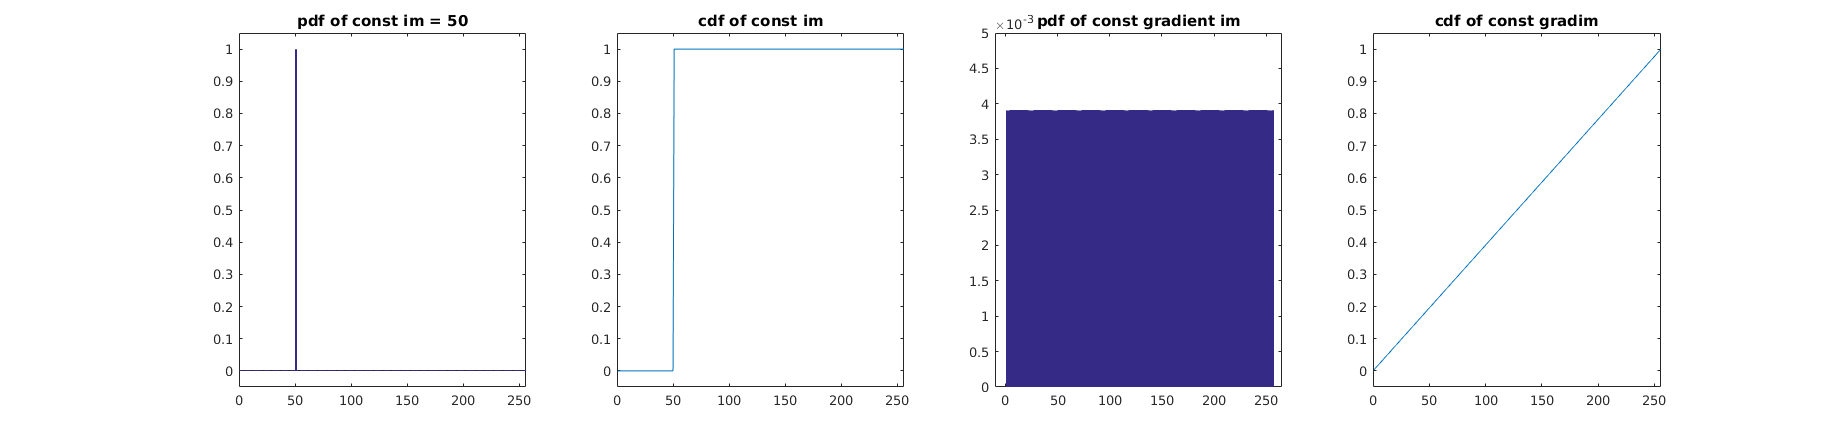
\includegraphics[width=\linewidth]{./1_2a.png}
  \caption{Normalised PDF and CFD in constant / constant gradient greyscale image}
  \label{fig:1.2}
\end{figure}

\newpage
\subsection{1.3.}
% \textit{``In the discrete setting, implement a MATLAB function that, to a given histogram of a grayscale image, computes its cumulative histogram (you may use MATLAB’s cumsum function and normalize the expression). Display it for the image pout.tif. What do the regions of fast increase of the function correspond to? And what about its flat regions?''}\\

The regions of fast increase of the function corresponds to high counts of pixel intensities and the flat regions corresponds to low counts (or no counts) of pixel intensities.

\begin{figure}[h]
  \centering
  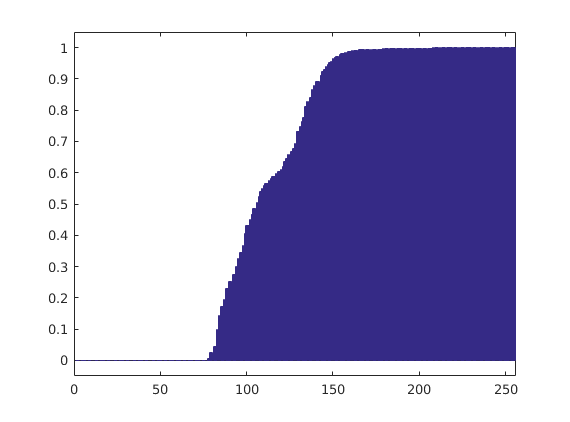
\includegraphics[width=\linewidth]{./1_3.png}
  \caption{Normalised Cumulative Histogram (cdf(h))}
  \label{fig:1.3}
\end{figure}

\begin{figure}[h!]
  \begin{lstlisting}[caption='Code to display Cumulative Histogram']
function [ cs ] = cdf(pdf)
  % pdf is a histogram
  c = double(cumsum(pdf));
  cs = c / c(end);
end

function cs = cumhist(fname)
  I = imread(fname);  % load image
  h = imhist(I);      % get histogram
  ncs = cdf(h);       % calculate 'normalized cumulative sum'
  % display the resulting array
  bar(ncs); axis([0 256 -0.05 1.05]);
end\end{lstlisting}
\end{figure}

\newpage
\subsection{1.4.}
% \textit{``Given an image I and its CDF C, write a matlab routine that computes the floating-point image C(I) such that the intensity at each pixel (i, j) is C(I(i, j))''}\\

The function takes an input image In and its CDF C, and for every pixel location (i,j) output the value C(In(i,j)), which is the CDF entry for the intensity IN(i,j)
\begin{figure}[h!]
  \begin{lstlisting}[caption='Code to compute cdf image']
function Out = fun14(In, C)
In = double(In);
Out = In;
[n,m] = size(In);
for i = 1 : n
    for j = 1 : m
        Out(i,j) = C(In(i,j));
    end
end
end
\end{lstlisting}
\end{figure}
Figure \ref{fig:1.4} shows the original image to the right and the output image after being run throught fun14. We can see how the intensities get brighter, this makes sense, since the CDF for the value 20, will be higher then 20, since it comulative of the previous entries.
\begin{figure}[h!]
  \centering
  \includegraphics[width=1\textwidth,, clip=true]{fig14.jpg}
  \caption{Original image and the image where I(i,j) = CDF(I(i,j))}
  \label{fig:1.4}
\end{figure}

\newpage
\subsection{1.5.}
% \textit{``Is the CDF invertible in general and why? To overcome the problem of non-invertibility for histogram matching (cf 3.4.5), we can consider instead a pseudo-inverse. For any CDF function f defined on the integer set {0, .., 255}, we define its pseudo-inverse $f^{-1}$ as follows : $f^{-1} (l) = min{s | f (s) \geq l}$,  where $l \in [0, 1]$. Write and add in your report a MATLAB routine that computes the pseudo-inverse of any given CDF (you may use MATLAB find and min functions)''}

The CDF is not invertible in general, because the inverse isn't a function. Take the example from \autoref{fig:1.3}, because it has a vertical line, it cannot pass the vertical line test. Also, one can see that as no values below the constant exist, $cdf(v)=0$, for $0<v<c$ and $cdf^{-1}(v) = \frac{1}{0}$ and division by zero is an illegal operation.

The pseudo inverse proposed in the assignment text is implemented as follows:
\begin{figure}[h!]
  \begin{lstlisting}[caption='cdf pseudo-inverse implementation']
function [ pseudo_inverse ] = cdfpinv( cdf, l )
  % find the cdf values larger than l, and return the least of them
  pseudo_inverse = min( find(cdf >= l) );
end\end{lstlisting}
\end{figure}

\subsection{1.6.}
% \textit{``Based on equation (3.25) and on the two previous questions, implement your own MATLAB procedure to perform histogram matching between two images and show results. Plot and compare the cumulative histograms of the original image, the target and the one obtained by histogram matching.''}\\

The \textit{histmatch} procedure is implemented in matlab, and the results are shown in \autoref{fig:1.6} and \autoref{fig:1.7}.


\begin{figure}[h!]
  \centering
  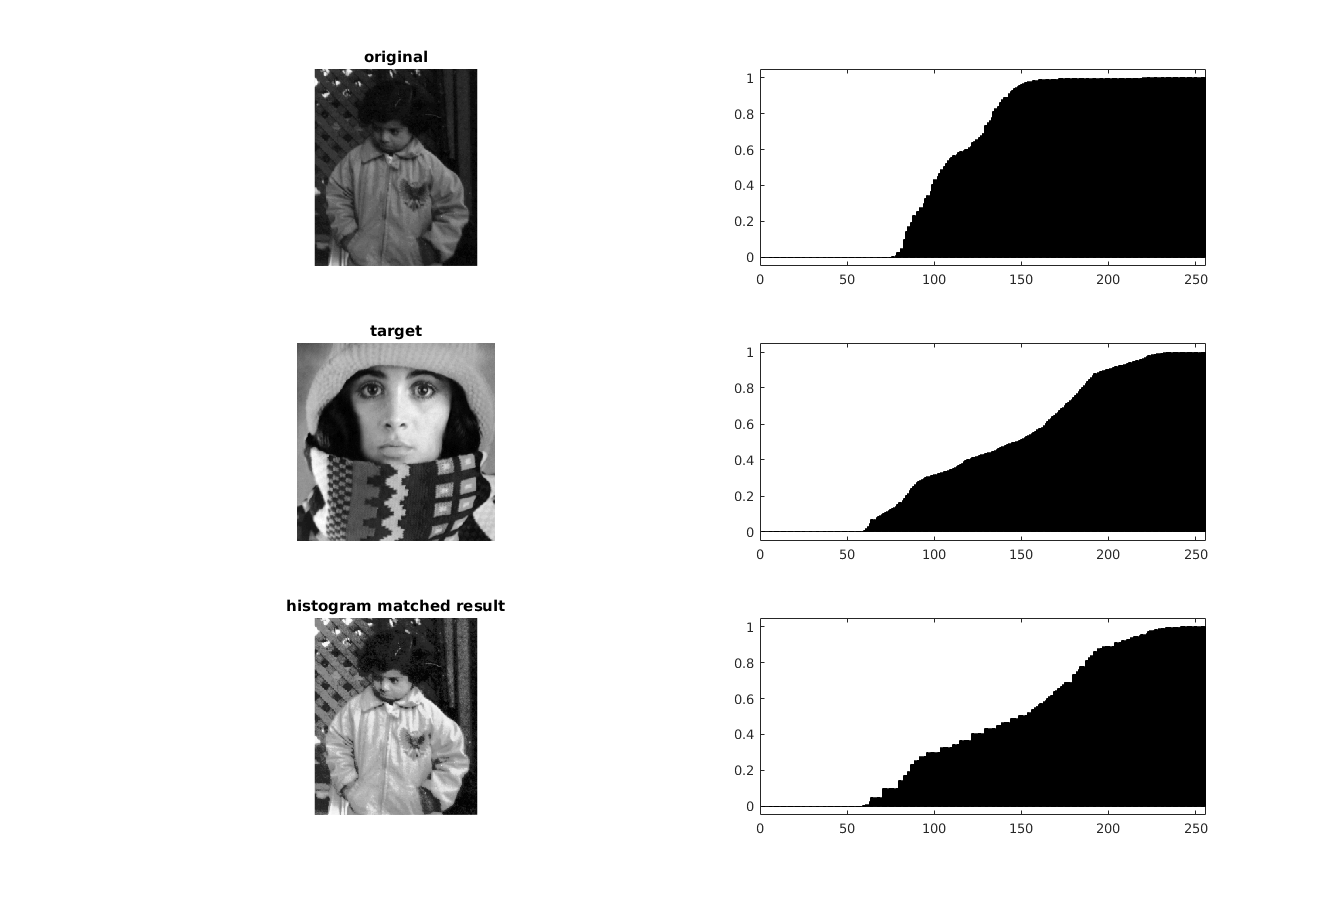
\includegraphics[width=1\textwidth, clip=true]{./1_6.png}
  \caption{Image 'pout.tif' matched with the histogram characteristics of the 'trui.png' image}
  \label{fig:1.6}
\end{figure}

\begin{figure}[h!]
  \begin{lstlisting}[caption='cdf histmatch implementation']
function [ Ix_matched_to_Iz ] = histmatch(I_x, I_z)
  Cx = cdf(pdf(I_x));
  Cz = cdf(pdf(I_z));
  Czinv = uint8(pinv( Cz, Cx ));
  Ix_matched_to_Iz = applymapping(I_x, Czinv);
end
im        = imrea\tilde{I}_1d('images/pout.tif');
targetim  = imread('images/trui.png');
matched   = histmatch(im, targetim);\end{lstlisting}
\end{figure}



\newpage
\subsection{1.7.}
% \textit{``Apply it in the particular case where the target cumulative histogram is the one corresponding to a constant histogram. Compare the result to MATLAB histeq built-in function.''}\\

The histmatch function applied to the \texttt{pout.tif} image and the constant histogram. It seems that the effect is equal to the matlab \textit{histeq} build-in function.

\begin{figure}[h!]
  \centering
  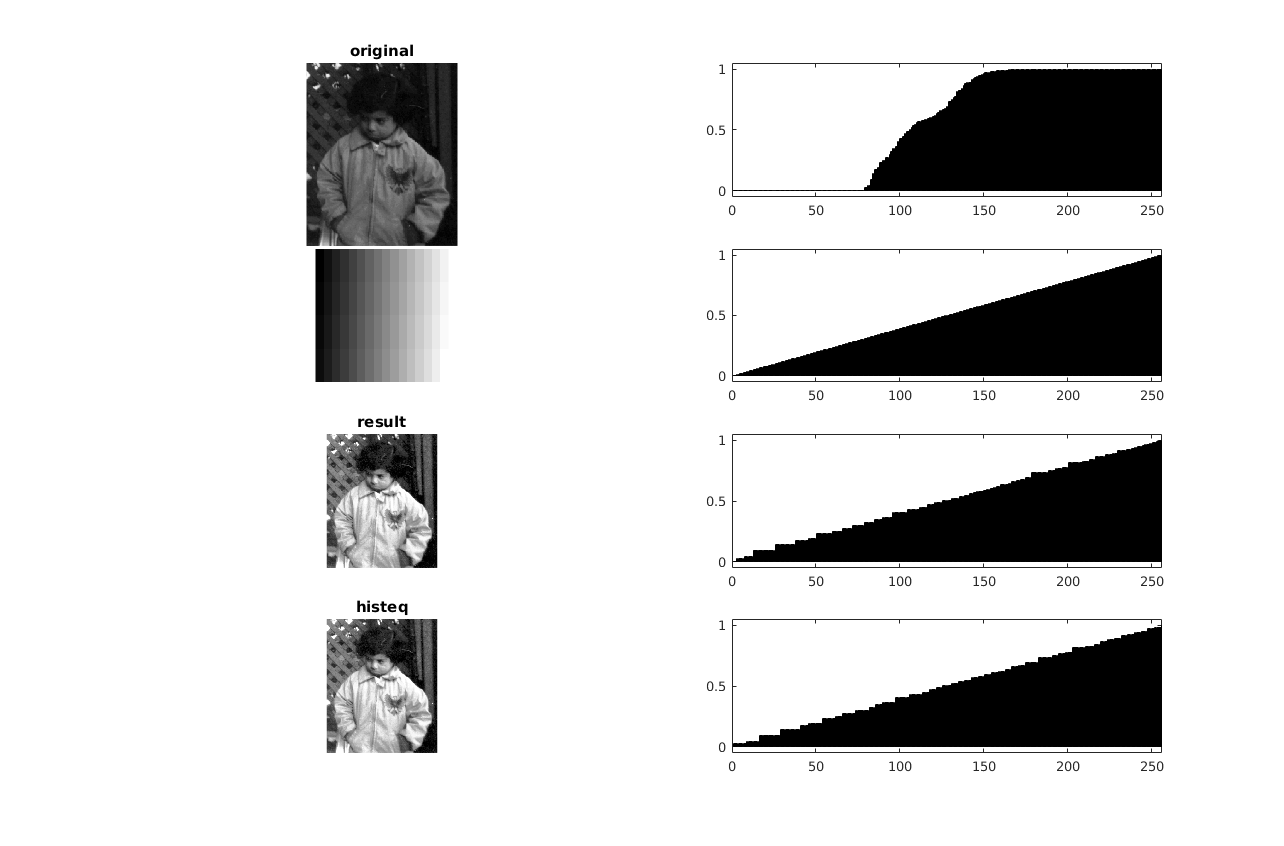
\includegraphics[width=1\linewidth, trim={40 40 40 30 }, clip=true]{./1_7.png}
  \caption{Image 'pout.tif' matched with uniform pdf image, and compared to matlab histeq}
  \label{fig:1.7}
\end{figure}

\begin{figure}[h!]
  \begin{lstlisting}[caption='application of histmatch to constant histogram image']
im        = imread('images/pout.tif');
targetim  = reshape(uint8(0:255),16,16);  % constant gradient (histogram)
matched   = histmatch(im, targetim);
he        = histeq(im);

plots...\end{lstlisting}
\end{figure}

\newpage
\subsection{1.8.}
% \textit{``Let I 1 and I 2 be two images with cumulative histograms C 1 and C 2 . Let’s introduce : $\phi = \frac{1}{2} \left( C_1^{(-1)} + C_2^{(-1)} \right) $ and the images $\tilde{I}1 = \phi(C1 (I1))$ and $\tilde{I}2 = \phi(C2 (I2 )) $ called the midway specifications of I1 and I2. If I1 and I2 are two constant images with respective values a and b, prove that the midway specifications are both equal to the constant image (a+b)/2? Is the cumulative histogram of the midway specifications equal to the average of the cumulative histograms ? ''}\\

\subsubsection{1.8.1.}
NEW
We have $  \phi = \frac{1}{2} (C_1^{-1} + C_2^{-1})$, inserting
\begin{align*}
  \tilde{I}_1 &= \phi(C_1(I_1)) &&&  \tilde{I}_2 &= \phi(C_2(I_2))\\
  \tilde{I}_1 &= \frac{1}{2} \left( C_1^{(-1)}(C_1(I_1)) + C_2^{(-1)}(C_1(I_1)) \right) &&&
  \tilde{I}_2 &= \frac{1}{2} \left( C_1^{(-1)}(C_2(I_2)) + C_2^{(-1)}(C_2(I_2)) \right)\\
  \tilde{I}_1 &= \frac{1}{2} \left( I_1 + C_2^{(-1)}(C_1(I_1)) \right) &&&
  \tilde{I}_2 &= \frac{1}{2} \left( C_1^{(-1)}(C_2(I_2)) + I_2) \right)\\
\end{align}
Remembering definition 3.25
$$
f(x) = C_z^{-1}(C_x(x))
$$
Where z = f(x), we can thus use this to get $C_2^{(-1)}(C_1(I_1)) = I_2$ and $C_1^{(-1)}(C_2(I_2)) = I_1$ substitution in this in gets us
\begin{align*}
  \tilde{I}_1 &= \frac{1}{2} \left( I_1 + I_2 \right) &&&
  \tilde{I}_2 &= \frac{1}{2} \left( I_1 + I_2 \right)\\
\end{align}
We have proved that for constant images the midway specification is equal to the constant $\frac{a+b}{2}$ where a and b are the two images.


\subsubsection{1.8.2.}
\begin{figure}[h!]
  \centering
  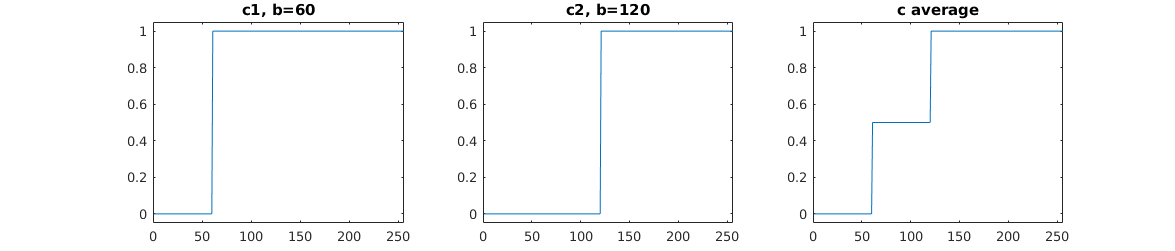
\includegraphics[width=\linewidth, trim={10 0 0 0 }, clip=true]{./1_8.png}
  \caption{Images with averaged cumulative histograms}
  \label{fig:1.8}
\end{figure}

Assuming application of histmatch to constant histogram that $\tilde{I}_1 = \tilde{I}_2$, \autoref{fig:1.8} shows that the cumulative histogram of the midway specifications cannot be equal to the average of the cumulative histograms. The reason is that there is clearly 2 'jumps' on the average cdf, and there would be only one jump if $\tilde{I}_1 = \tilde{I}_2$.

\newpage
\subsection{1.9.}
% \textit{``Write a MATLAB function that computes the midway specifications of two images. Show the result on the images movie.flicker1.tif and movie.flicker2.tif located in the Test Images folder (convert them to grayscale) which corresponds  to two successive frames of the 1948 movie "Les aventures des Pieds-Nickeles" (copyright Marc Sandberg). How would you generalize midway equalization to an arbitrary number of images ?''}\\

\autoref{fig:1.9ab} shows the two original images in the top row, and it is seen that the leftmost seems darker, which is confirmed by the cdf displayed underneath the image.
In the second row, the two images are 'maidwayed' with respect to the other, and seeming at a similar intensity level on visual inspection, which is confirmed by the cdf's below, which are both very similar, and both looks like a midway compromise of the two top ones.

\begin{figure}[h!]
  \centering
  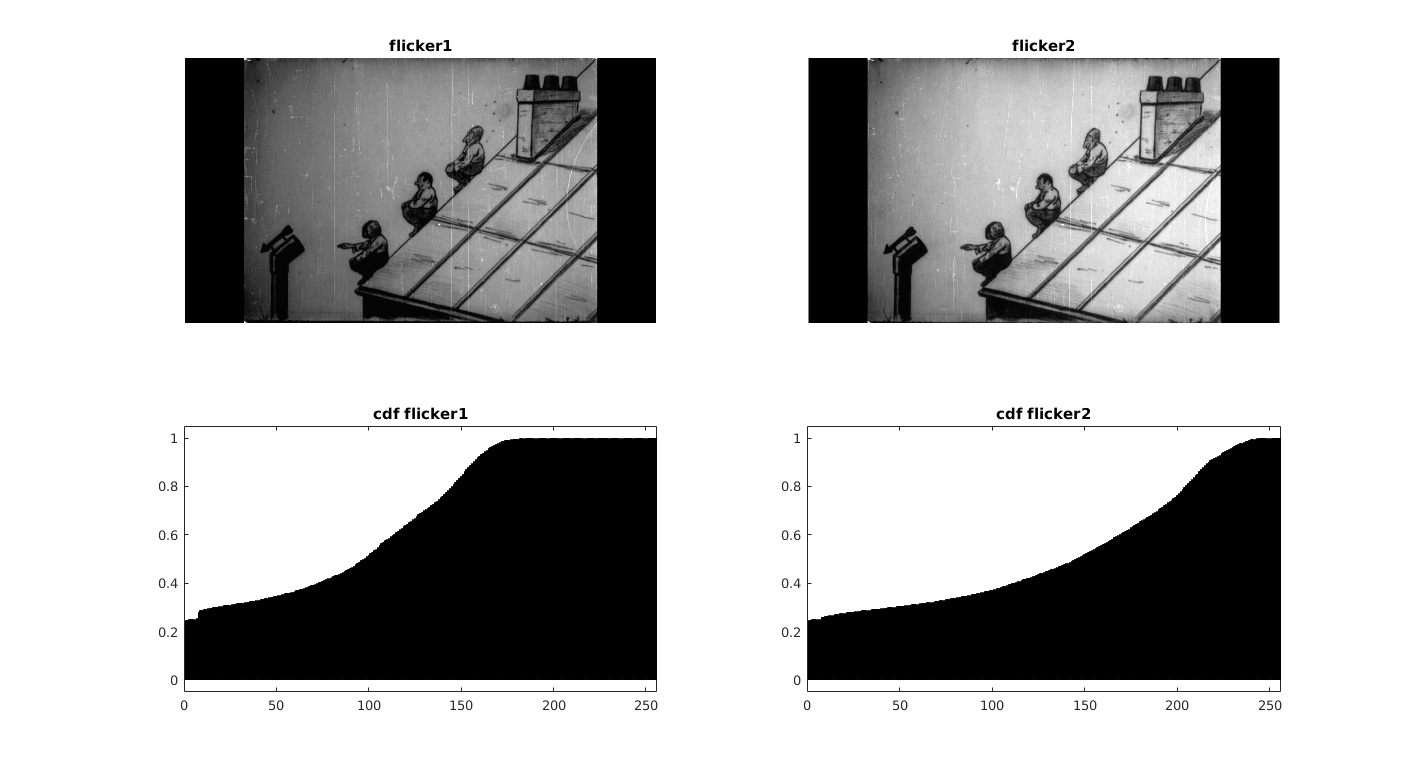
\includegraphics[width=0.8\linewidth, trim={35mm 0mm 35mm 0mm }, clip=true]{./1_9a.png}
  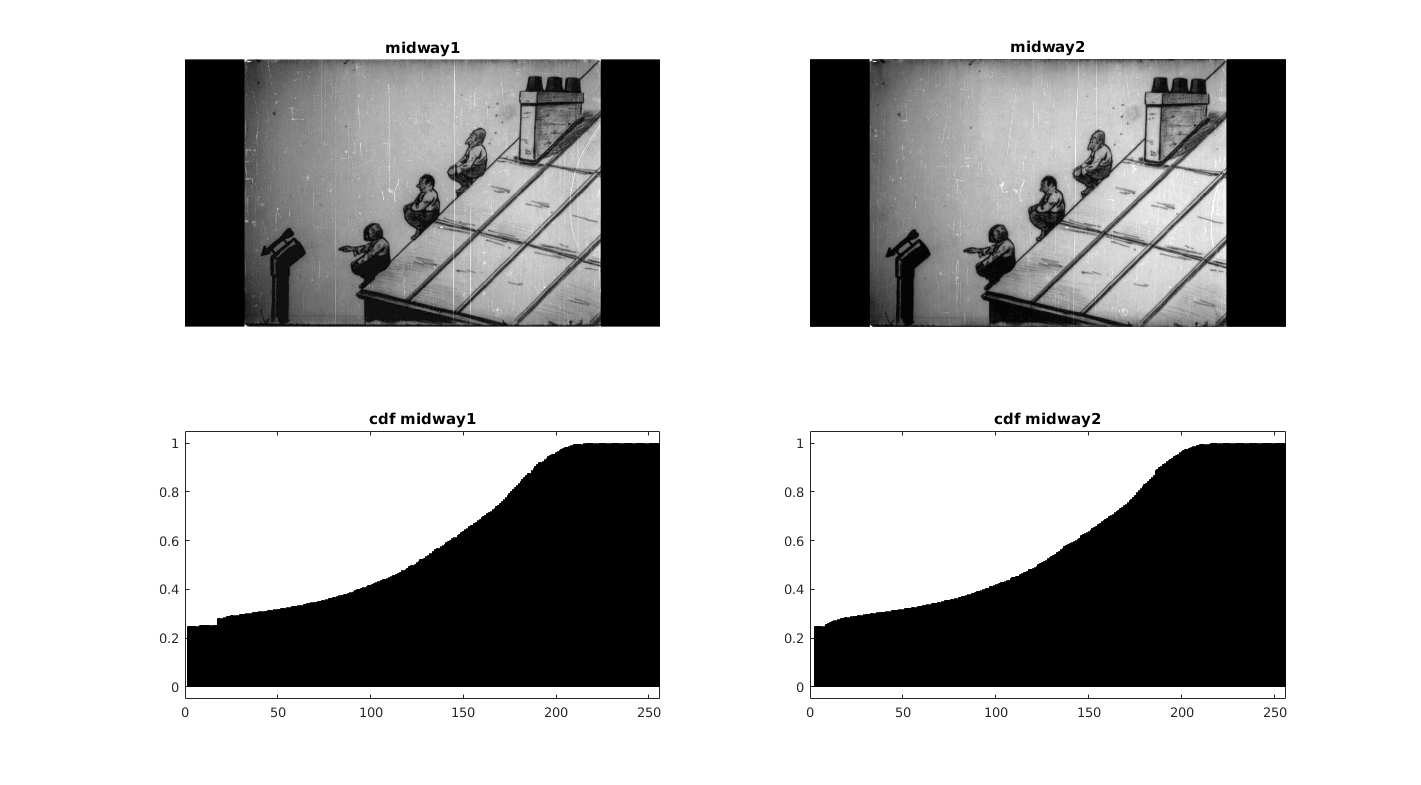
\includegraphics[width=0.8\linewidth, trim={35mm 0mm 35mm 0mm }, clip=true]{./1_9b.png}
  \caption{Original image frames, and midwayed image frames}
  \label{fig:1.9ab}
\end{figure}

\autoref{fig:1.9c} shows the absolute difference in the images, which is of course big along the edges of movement in the two different frames, but further it is evident that the intensity of the original frames differ very much on average, and this difference is almost totally gone in the 'midway'ed' imageset.

\begin{figure}[h!]
  \centering
  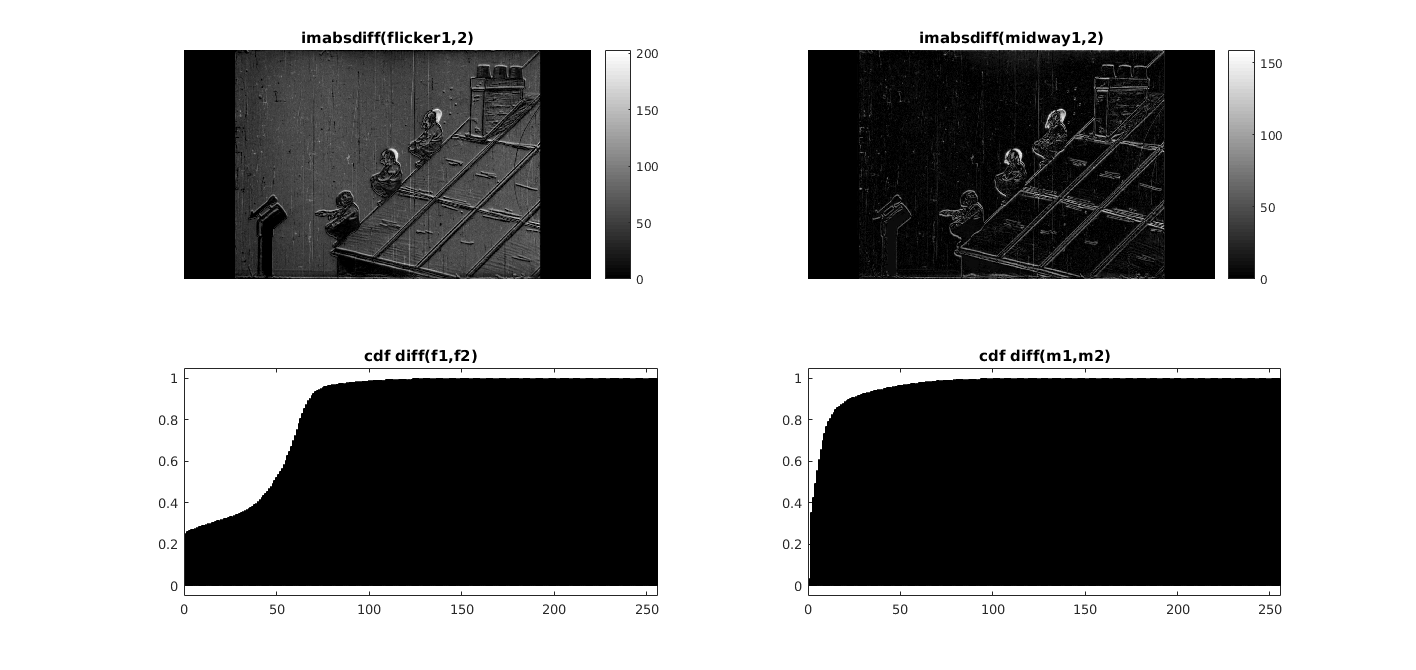
\includegraphics[width=0.8\linewidth, trim={110 0 110 0 }, clip=true]{./1_9c.png}
  \caption{Absolute difference of originals vs midwayed image frames}
  \label{fig:1.9c}
\end{figure}

To generalize the midway equalization, to an arbitrary number $n$ of images, it is written:
$$ \phi = \frac{1}{n} \sum_{i=1}^{n} C^{(-1)}_i $$
The matlab function IS generalized, it currently returns an midway'ed version of the first image argument, 'averaged' with them all.

\begin{figure}[h!]
  \begin{lstlisting}[caption='Midway function and its application.']
function out = midway(Is)
  % general midway function, taking up to n images, usage midway({im_1, .., im_n})
  phi = zeros([1 256]);  n  = length(Is);
  I   = Is{1};           CI = cdf(pdf(I));
  for i=1:n
      C    = cdf(pdf(Is{i}));
      Cinv = pinv(C, CI);
      phi  = phi + Cinv;
  end
  phi = uint8( phi / n );
  out = applymapping(I, phi);
end

im3  = midway({im1, im2});
im4  = midway({im2, im1});

d12 = imabsdiff(im1,im2);
d34 = imabsdiff(im3,im4);\end{lstlisting}
\end{figure}

\clearpage

\section{2. Image filtering and enhancement}

\subsection{2.1.}
The approximation for the x value uses the difference between the pixel before and the pixel after. The y value is calculated the same way. This results in the kernel:
$$
K =
\begin{bmatrix}
  -1 & 0 & 1
 \end{bmatrix}
$$

The imfilter function can either use correlation or convolution, the default is correlation. Correlation and convolution are almost the same, but convolution flips the kernel, on both axis. So the resulting kernel for the simle approximation approach with convolution is
$$
K =
\begin{bmatrix}
  1 & 0 & -1
 \end{bmatrix}
$$
For kernels like gaussians, which are symmetrical around the center, it does not matter which we choose to use, since kernels that will run over the image for the correlation and convolution will be the same.
\subsection{2.2}

The kernel in 4.5.2.1 shows the kernel for the x derivative, and thus these will be used for discussion. Instead of just looking at the pixel to the right and the left, we also use the information about the row above and below. By using the row above and below, we don't interpret a single noise pixel as being part of an edge, since the pixels below and above does not indicate that there is a continued edge. This makes noise get lower values than real edge, which spanned multiple rows. The same logic is applied for the y derivative, where we look at the derivatives and both sides. Sobel weighs the current row's pixels higher the the ones below and above. Where Prewitt weighs them equally.

\subsection{2.3.}
Figure \ref{fig:2_3_0} shows the eight.tif image with both salt and pepper noise, and gaussian noise, filtered with mean and median filter. The first column shows the image with salt and pepper noise with a mean filter, the second column is the image with gaussian noise filtered with mean filter. The third column shows the image with salt and pepper noise, filtered with a median filter and the fourth column shows the image with gaussian noise, with a median filter. The first row has a windows size of 3, the second window size of 5 and the third a window size of 7. Looking at the first column we can see how increasing windows size improves the denoising, but also the edge blur a bit. In the second column we see again how increasing the windows size improves the denoising. For the median filter the salt and pepper in column 3 is as good as gone in the first image, with windows size 3, increasing the window size only blurs the image a bit more, and makes the background brighter. In column 4 with gaussian noise we see that the increase in window size improves the denoising, while blurring the image, about as much as with the mean filter.

\begin{figure}[!ht]
    \centering
    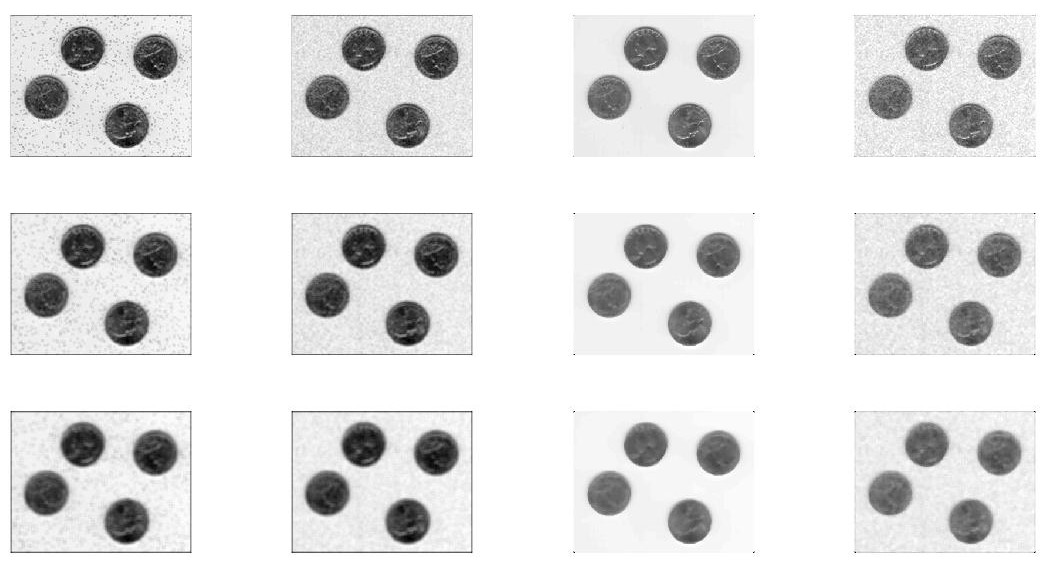
\includegraphics[width=1\textwidth]{fig23_0.jpg}
    \caption{mean and median filter on salt/pepper noise and on gaussian noise for different window sizes}
    \label{fig:2_3_0}
\end{figure}

Figure \ref{fig:2_3} shows the computational cost for increasing window sizes. The blue line is median filter and the red is mean filter. As we can see, the median filter is generally more expensive to use, compared to the mean filter. Another thing to notice is that the median filter has a lower computational cost when the windows size is odd. It also looks like the median filter spikes more, and increases in computational cost, when N becomes bigger, see when $N \geq 21$ on the graph, compared to the mean filter, which seems to be increasing at a steady pace.

\begin{figure}[!ht]
    \centering
    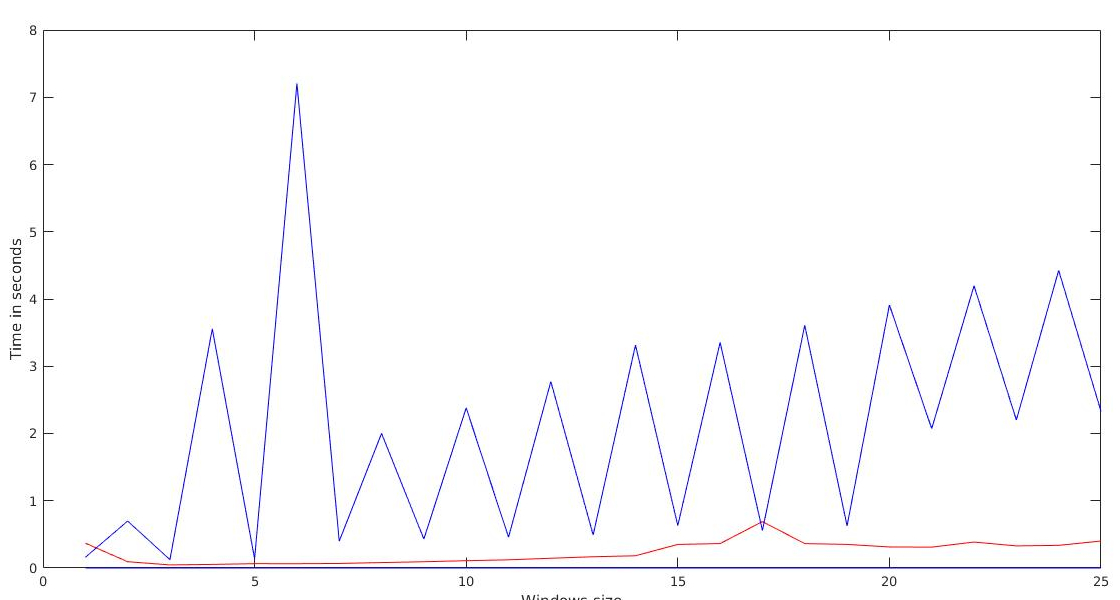
\includegraphics[width=1\textwidth]{fig23.jpg}
    \caption{The computational cost of doing mean filter and median filter, based on window size.}
    \label{fig:2_3}
\end{figure}

\clearpage

\subsection{2.4.}
Figure \ref{fig:2_4} shows the eight.tif, with salt and pepper noise, filtered with a gaussian kernel where $\sigma = 5$, with windows size in the range 3:19, with increments of 2, to keep the kernel diameter odd. We can see how the difference between image 5 and image 8, are less noticeable then the difference between image 2 and image 5. This is because with a smaller windows, the image is blurred less. At some point the windows is so big, that the values furthest away from the center are so small, that their weights are neglect able, thus increasing the windows size show no noticeable difference. And that is why its easier to see the difference between image 2 and 5 then image 5 and 8.

\begin{figure}[!ht]
    \centering
    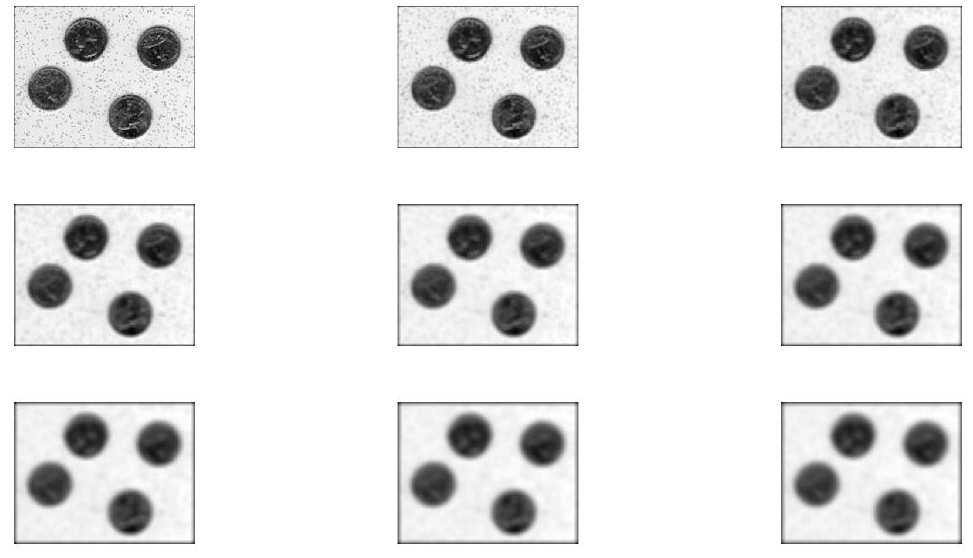
\includegraphics[width=1\textwidth]{fig24.jpg}
    \caption{9 Images with inceasing windows size starting at 3 ending at 19.}
    \label{fig:2_4}
\end{figure}

\clearpage

\subsection{2.5.}

Figure \ref{fig:2_5} show the eight.tif, with salt and pepper noise, filtered with a gaussian filter, with increasing $\sigma$ starting at 1 and ending at 17, in incremental steps of 2. The windows size N is 3*sigma + 1, and then rounding up to nearest odd integer. What we can see is that increasing $\sigma$ and windows size, rapidly improves the noise reduction, but also blurs the edges to an equal extend. In image 4, the noise is as good as gone, so from there on, the only difference is just that the edges in the following images are more blurred out. So increasing the $\sigma$ and windows size does makes the filter more effective at removing noise, but also makes finding edges harder. The noise removal is not something that improves the larger $\sigma$, since when sigma = 7 and window size = 23, the noise is gone, and we can't do better than remove it.
\begin{figure}[!ht]
    \centering
    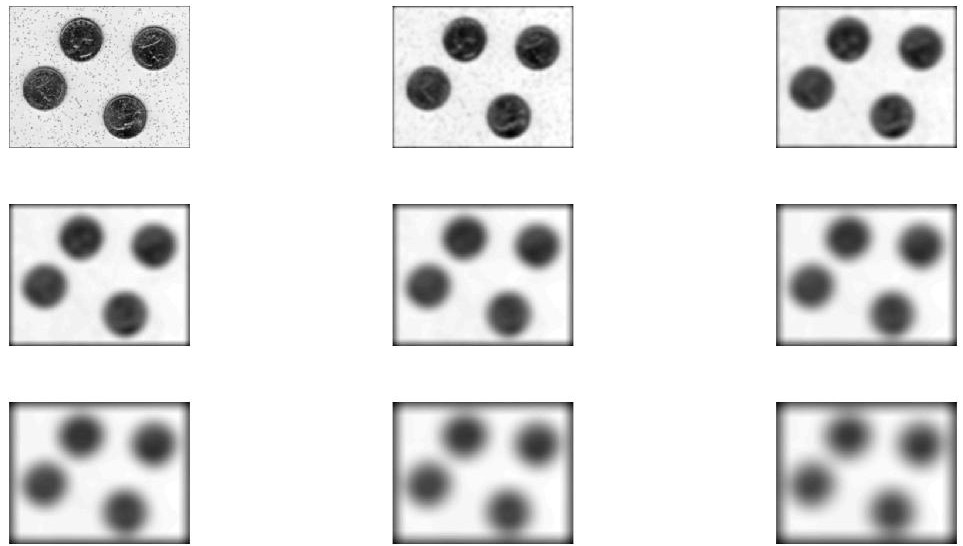
\includegraphics[width=1\textwidth]{fig25.jpg}
    \caption{9 Images with increasing sigma and windows size starting at sigma = 1 and ending at sigma = 17, with increments of 2.}
    \label{fig:2_5}
\end{figure}

\clearpage

\section{3 Bonus questions}

\subsection{3.1.}

The bilateral filter is not linear, because of the non-linear dependency on the weights $w$. The term that differs from the usual Gaussian filter is the range intensity difference smoothing term $g_\tau$. The interpretation of the $\tau$ parameter is that it is the intensity smoothing parameter, which for low values weighs intensity differences higher and for high values weighs intensity differences the same. Bilateral filtering becomes usual Gaussian filtering in the limit of $\tau$ as it approaches $\infty$, because $g_\tau$ approaches 1.

\subsection{3.2.}

\lstinputlisting{bilateral_filtering.m}\\

The function first pads the image with zeroes to avoid out of bounds exceptions. It then computes the spatial gaussian filter. Finally it computes the filtered image.\\
\\
\subsection{3.3.}

\begin{figure}[h]
\centering
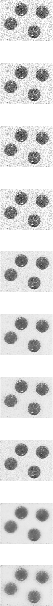
\includegraphics{A3_3_1.png}

\includegraphics{A3_3_2.png}
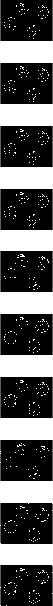
\includegraphics{A3_3_3.png}

\includegraphics{A3_3_4.png}
\caption{Bilateral filtering and edge detection applied to \textit{eight.tif} corrupted by gaussian noise, for various $\sigma$ and $\tau$.}
\end{figure}

Bilateral filtering and edge detection applied to \textit{eight.tif} corrupted by gaussian noise, for various $\sigma$ and $\tau$ can be seen in figure 13. The first column is the filtered image, the second is \textit{Sobel} edge detection, the third is \textit{Prewitt} edge detection, and the fourth is \textit{Zero-cross} edge detection. The image in the first row and the first first column is the original unfiltered image. $\sigma = 1$ in rows 2, 5, and 8, $\sigma = 9$ in rows 3, 6, and 9, and $\sigma = 17$ in rows 4, 7, 10. $\tau = 10$ in rows 2, 3, and 4, $\tau = 50$ in rows 5, 6, and 7, and $\tau = 90$ in rows 8, 9, and 10. The window size is three times $\sigma$.

The reduction in noise is increased as $\tau$ and $\sigma$ is increased, but so is the amount of blurring. The best settings amongst those applied seems to be $\sigma = 9$ and $\tau = 50$, which correspond to row 6.

\clearpage
\appendix
\section{helper methods}
\begin{figure}[h!]
  \begin{lstlisting}[caption='applies a mapping']
function out = applymapping(in, map)
    % apply the mapping
    [cs rs] = size(in);
    out = uint8(zeros([cs rs]));
    for r = 1:rs
        for c = 1:cs
            out(c,r) = map( in(c,r)+1 );
        end
    end
end\end{lstlisting}
\end{figure}

\end{document}
